\section{Theoretical Analysis}
\label{sec:analysis}

\paragraph{}
In this section, we can find the results of each topic required in the theoretical analysis. The numeric results or graphics are presented alongside a short explanation of the interpretation of the problem. All of the results were obatined usig GNU octave and the section is dividid in six different subsections - Subsection ~\ref{subsec:first_topic}, Subsection ~\ref{subsec:second_topic}, Subsection ~\ref{subsec:third_topic}, Subsection ~\ref{subsec:fourth_topic}, Subsection ~\ref{subsec:fifth_topic} and Subsection ~\ref{subsec:sixth_topic} -, one for each topic of the theoretical analysis.

\subsection{Theoretical - Topic I}
\label{subsec:first_topic}

\paragraph{}
We start to apply the Node Voltage Method by starting to identify the nodes of the circuit. In this case, our circuit has 8 nodes and each one has a node voltage designated $V_1$, $V_2$, $V_3$, $V_4$, $V_5$, $V_6$, $V_7$ and $V_8$, according to the related node. Then, we apply the KCL to each one of the nodes.

\[
\left\{\begin{matrix}
Node 1: V_1 = V_S\\
Node 2: I_1 + I_2 = I_3\\
Node 3: I_B = I_2\\
Node 4: V_4 = 0\\
Node 5: V_5 -V_8 = V_D\\
Node 6: I_C + I_B + I_5 = 0\\
Node 7: I_D = I_7\\
Node 8: V_5 -V_8 = V_D\\
\end{matrix}\right.
\]

\paragraph{}
After that, we rewrite it into an equivalent system defining the currents in terms of node voltages.

\[
\left\{\begin{matrix}
Node 1: V_1 = V_S\\
Node 2: \frac{V_1-V_2}{R_1} + \frac{V_3-V_2}{R_2} = \frac{V_2-V_5}{R_3}\\
Node 3: I_B = \frac{V_3-V_2}{R_2}\\
Node 4: V_4 = 0\\
Node 5: V_5 -V_8 = K_D*I_D\\
Node 6: I_C + I_B + \frac{V_6-V_5}{R_5} = 0\\
Node 7: I_D = \frac{V_7-V_8}{R_7}\\
Node 8: V_5 -V_8 = V_D\\
\end{matrix}\right.
\]

\paragraph{}
Now, we have a system of 6 equations (note that applying KCL to node 5 and node 8 generate the same exact equation). Between these two nodes, the circuit presents a voltage source $V_D$. Therefore, to obtain another equation to add to the system, we need to consider a supernode that includes both node 5 and node 8 and, after that, apply KCL to the supernode we just created.

\paragraph{}
We obtain another equation: $ I_3 + I_5 + I_C + I_D = I_4 $.

\paragraph{}
Once again, we define the currents in terms of node voltages and obtain an equivalent equation: $ \frac{V_2-V_5}{R_3}+\frac{V_6-V_5}{R_5} + I_C + I_D = \frac{V_5}{R_4} $.

\paragraph{}
At this point, we have a system with 7 equations. However, besides the node voltages $V_1$, $V_2$, $V_3$, $V_5$, $V_6$, $V_7$ and $V_8$, we still have two more variables to determine its value, $I_B$ and $I_D$ (note that $I_C = 0 V $ when $t < 0$). So, we need to find two more equations to complete our system. We have to define the missing value currents in terms of node voltages and get the two extra equations.

\[
\left\{\begin{matrix}
I_B = (V_2-V_5)*K_B \\
I_D = \frac{0-V_7}{R_6} \\
\end{matrix}\right.
\]

\paragraph{}
This takes us to our final system of equations, with 10 equations to find the values of 10 variables.

\[
\left\{\begin{matrix}
V_1 = V_S\\
\frac{1}{R_1}V_1 + (-\frac{1}{R_1} -\frac{1}{R_2} -\frac{1}{R_3})V_2 +\frac{1}{R_2}V_3 + \frac{1}{R_3}V_5 = 0
I_B - \frac{1}{R_2}V_3 +\frac{1}{R_2}V_2 = 0\\
V_5 - V_8 - K_D*I_D = 0\\
I_B + \frac{1}{R_5}V_6 -\frac{1}{R_5}V_5= 0\\
I_D - \frac{1}{R_7}V_7 + \frac{1}{R_7}V_8 = 0\\
I_D + \frac{V_2-V_5}{R_3} + \frac{V_6-V_5}{R_5} - \frac{V_5}{R_4} = 0\\

I_D + \frac{1}{R_3}V_2 + (-\frac{1}{R_3} -\frac{1}{R_4} -\frac{1}{R_5})V_5 + \frac{1}{R_5}V_6 = 0\\

I_B - -K_B*V_2 + K_B*V_5 = 0\\
I_D + \frac{V_7}{R_6} = 0\\
\end{matrix}\right.
\]

\paragraph{}
We can transform this system of equations and put it into a matrix form, ready to be solved in GNU Octave.

\[
\begin{bmatrix}
1 & 0 & 0 & 0 & 0 & 0 & 0 & 0 & 0 & 0\\

\frac{1}{R_1} & -\frac{1}{R_1} -\frac{1}{R_2} -\frac{1}{R_3} & \frac{1}{R_2} & \frac{1}{R_3} & 0 & 0 & 0 & 0 & 0 & 0\\

0 & \frac{1}{R_2} & -\frac{1}{R_2} & 0 & 0 & 0 & 0 & 1 & 0 & 0\\

0 & 0 & 0 & 1 & 0 & 0 & -1 & 0 & 0 & -K_D\\

0 & 0 & 0 & -\frac{1}{R_5} & \frac{1}{R_5} & 0 & 0 & 1 & 1 & 0\\

0 & 0 & 0 & 0 & 0 & \frac{1}{R_7} & -\frac{1}{R_7} & 0 & 0 & -1\\

0 & -K_B & 0 & K_B & 0 & 0 & 0 & 1 & 0 & 0\\

0 & \frac{1}{R_3} & 0 & -\frac{1}{R_3}-\frac{1}{R_4}-\frac{1}{R_5} & \frac{1}{R_5} & 0 & 0 & 0 & 1 & 1\\

0 & 0 & 0 & 0 & 0 & \frac{1}{R_6} & 0 & 0 & 0 & 1\\

0 & 0 & 0 & 0 & 0 & 0 & 0 & 0 & 1 & 0 \\
\end{bmatrix}
\begin{bmatrix}
V_1\\
V_2\\
V_3\\
V_5\\
V_6\\
V_7\\
V_8\\
I_B\\
I_C\\
I_D\\
\end{bmatrix}
=
\begin{bmatrix}
V_S\\
0\\
0\\
0\\
0\\
0\\
0\\
0\\
0\\
0\\
\end{bmatrix}
\]

\paragraph{}
These are the final values obtained with the application of the Node Voltage Method:

\begin{center}
   \begin{tabular}{|c||c|}
      \hline    
      \multicolumn{2}{|c|} {\bf Nodal Analysis Voltages [in Volts]} \\
      \hline
        
 Node Voltage 1 & 5.02924600001e+00 \\ \hline 
 Node Voltage 2 & 4.78354415384e+00 \\ \hline 
 Node Voltage 3 & 4.28814736170e+00 \\ \hline 
 Node Voltage 5 & 4.81753272504e+00 \\ \hline 
 Node Voltage 6 & 5.57990489781e+00 \\ \hline 
 Node Voltage 7 & -1.85471262435e+00 \\ \hline 
 Node Voltage 8 & -2.77162277031e+00 \\ \hline 
   \end{tabular}
 \end{center}

 %%%%%%%%%%%%%%%%%%%%%%%%%%%%%%%%%

\subsection{Theoretical - Topic II}
\label{subsec:second_topic}

\[
\left\{\begin{matrix}
v_s=0V\\
V_x=V_6-V_8\\
\end{matrix}\right.
\]

\paragraph{}
To analyze an RC circuit more complex than simple series (given that we are dealing with a complex electric circuit with different dependent sources), we can convert the circuit into a Thévenin equivalent, applying Thévenin's theorem. Then, we treat the capacitor as the "load” and reduce everything else to an equivalent circuit of one voltage source and one series resistor. After that, we are able to analyze what happens over time with the universal time constant formula. Our time constant for this circuit will be equal to the Thévenin' resistance, $R_{eq} $, times the capacitance $C$.

\begin{center}
   \begin{tabular}{|c||c|}
      \hline    
      \multicolumn{2}{|c|} {\bf Nodal Analysis Voltages [in Volts]} \\
      \hline
        
 Node Voltage 1 & 0.00000000000e+00 \\ \hline 
 Node Voltage 2 & 1.69330273904e+00 \\ \hline 
 Node Voltage 3 & 1.32728398106e+00 \\ \hline 
 Node Voltage 5 & 1.71841484072e+00 \\ \hline 
 Node Voltage 6 & 7.28976333729e+00 \\ \hline 
 Node Voltage 7 & -4.79175543809e-01 \\ \hline 
 Node Voltage 8 & -2.42286598296e-01 \\ \hline 
 Req, Equivalent Resistor & -4653.537219 \\ \hline 
 Time Constant & -0.004797 \\ \hline 
   \end{tabular}
 \end{center}
 
 where $ R_{eq} = \frac{V_x}{I_x} $ is expressed in Ohms $(\Omega)$ and \\
 the time constant $\tau$ is expressed in seconds (s). 
 %%%%%%%%%%%%%%%%%%%%%%%%%%%%%%%%%
 
\subsection{Theoretical - Topic III}
\label{subsec:third_topic}

\paragraph{}
The natural response tells us what the circuit does as its internal stored energy (the initial voltage on the capacitor, calculated in the previous topic, $V_x$) is allowed to dissipate. It does this by ignoring the forcing input and considering only the initial voltage and the equivalent resistance and time constant, determined in the previous topic.

\paragraph{}
$ v_n(t)=V_x e^{-\frac{t}{\tau}}=V_x e^{-\frac{t}{RC}} $

\begin{figure}[H] \centering
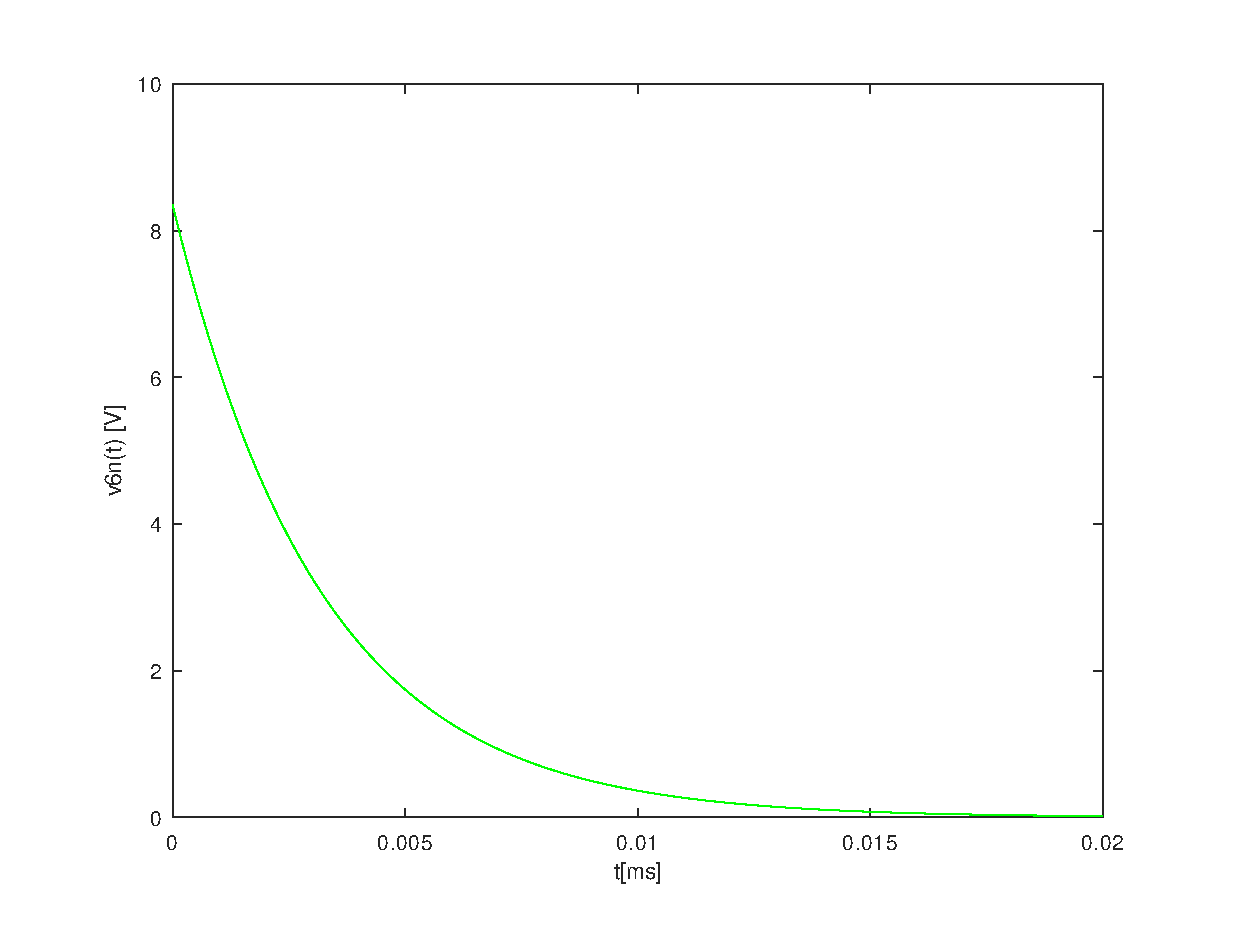
\includegraphics[width=0.6\textwidth]{natural.eps}
\caption{The natural solution, $V6_n(t)$, during time interval [0, 20] ms.}
\label{fig:theo_third}
\end{figure}

where $t$ is expressed in seconds (s) along the x-axis and \\
$V6_n(t)$, the natural solution, is expressed in Volts (V) along the y-axis.


 %%%%%%%%%%%%%%%%%%%%%%%%%%%%%%%%%
 
\subsection{Theoretical - Topic IV}
\label{subsec:fourth_topic}

\paragraph{}
The forced response is where the output (the voltage on the capacitor) is going to end up in the long run after all stored energy eventually dissipates. This occors by ignoring the presence of energy storage elements (in our circuit analysis, it ignores the capacitor and its initial voltage, $V_x$). As suggested, plotting the amplitude and phase shift of a sinusoid in a complex plane, we get a complex number in polar form that we can apply to the circuit analysis: a phasor voltage source, $V_s$ = 1. Besides that, we also replaced $C$ with its impedance $Z_C=\frac{1}{\omega C}$.


\[
\left\{\begin{matrix}
f = 1 kHz = 1000 Hz \\
t = 20 ms = 0.020 s \\
\end{matrix}\right.
\]


\begin{center}
   \begin{tabular}{|c||c|}
      \hline    
      \multicolumn{2}{|c|} {\bf Nodal Analysis of Phasors [in Volts]} \\
      \hline
        
 Phasor of Node 1 & 6.12323399574e-17+i1.57079632679e+00 \\ \hline 
 Phasor of Node 2 & 5.78536935465e-17+i1.57079632679e+00 \\ \hline 
 Phasor of Node 3 & 5.10414916043e-17+i1.57079632679e+00 \\ \hline 
 Phasor of Node 5 & 5.83210704339e-17+i1.57079632679e+00 \\ \hline 
 Phasor of Node 6 & 8.26523333807e-02+i-1.42082340747e+00 \\ \hline 
 Phasor of Node 7 & -2.29152014669e-17+i-1.57079632679e+00 \\ \hline 
 Phasor of Node 8 & -3.40788140178e-17+i-1.57079632679e+00 \\ \hline 
   \end{tabular}
 \end{center}
  %%%%%%%%%%%%%%%%%%%%%%%%%%%%%%%%%
 
\subsection{Theoretical - Topic V}
\label{subsec:fifth_topic}

\paragraph{}
The natural response considers the internal initial conditions. The forced response considers the external inputs. Given that, we get the total response by summing the two responses, natural and forced. In fact, this is the principle of superposition in action (in the mathematical sense of differential equations).

\[
\left\{\begin{matrix}
v_t=v_n+v_f\\
f = 1 kHz = 1000 Hz \\
\end{matrix}\right.
\]

\begin{figure}[H] \centering
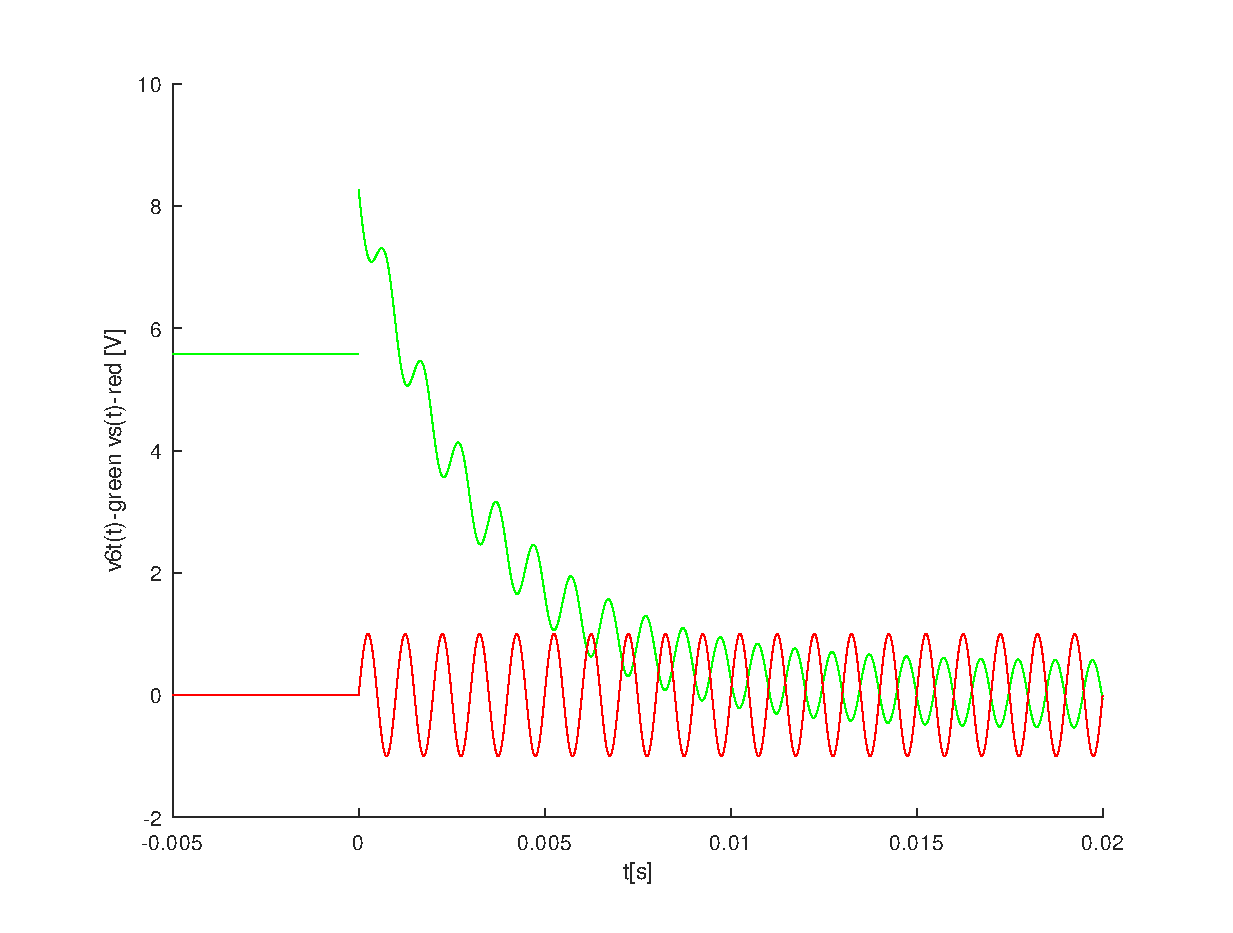
\includegraphics[width=0.6\textwidth]{total.eps}
\caption{The final total solution, $V6(t)$,  and $v_s(t)$ during time interval [-5, 20] ms.}
\label{fig:theo_fifth}
\end{figure}


Where $t$ is expressed in seconds (s) along the x-axis and 
$V6(t)$, the total solution, and $v_s$ are expressed in Volts (V) along the y-axis.

In the graphic above, it is ineteresting to note that, while the voltage emited by the source $V_s$ is constant, the node 6 will also have a constant voltage. This is because for $t<0$ the circuit will essentially behave as one of continuos current. After this time mark, the circuit reveals its alternate current nature and both the voltages of the source and of node 6 will vary sinousoidally.



  
  %%%%%%%%%%%%%%%%%%%%%%%%%%%%%%%%%

\subsection{Theoretical - Topic VI}
\label{subsec:sixth_topic}

\paragraph{}In this subsection, an analysis of the variation of the magnitude and phase of the phasors of $V_c$ $V_6$ and $V_s$ is made in function of the frequency. The first graphic presents the study of the variation of the magnitude and the second the study of the fase. In both graphics, the frequency $f$ in the x-axis varies from 0.1Hz to 1MHz


\[
\left\{\begin{matrix}
f =\in [0.1 , 1] MHz \\
v_c(f)=v_6(f)-v_8(f) \\
\end{matrix}\right.
\]


\begin{figure}[H] \centering
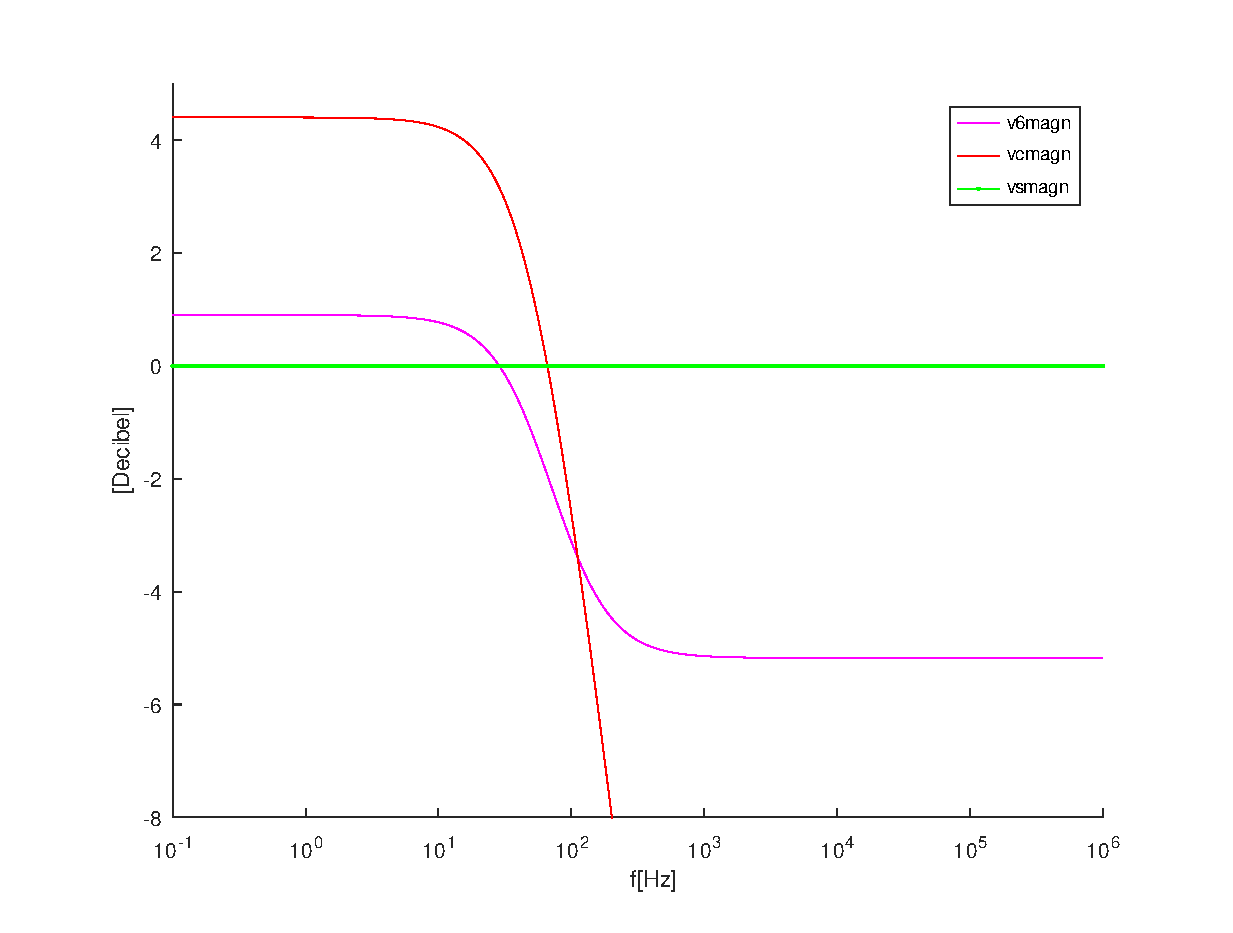
\includegraphics[width=0.6\textwidth]{magnitude.eps}
\caption{Magnitude of $v_s(f)$,  $v_c(f)$  and $v_6(f)$ during frequency interval [0.1 , 1] MHz.}
\label{fig:magnitudetheo}
\end{figure}

The frequency $f$ is expressed in Hertz (Hz) along the x-axis and 
the magnitude of $v_s(f)$,  $v_c(f)$  and $v_6(f)$ is expressed with a logscale decibel (dB) along the y-axis.\\
When looking at this graph, a couple of things are important to highlight. First, $V_s$ will always have magnitude 0 because, given that its absolute value is 1 and we are using a logscale, $log(1)=0$. Second, we also note that the $v_c$ graph line does not resemble the one that represents $v_6$. This is because the voltage of the node 8 will also vary. 


\begin{figure}[H] \centering
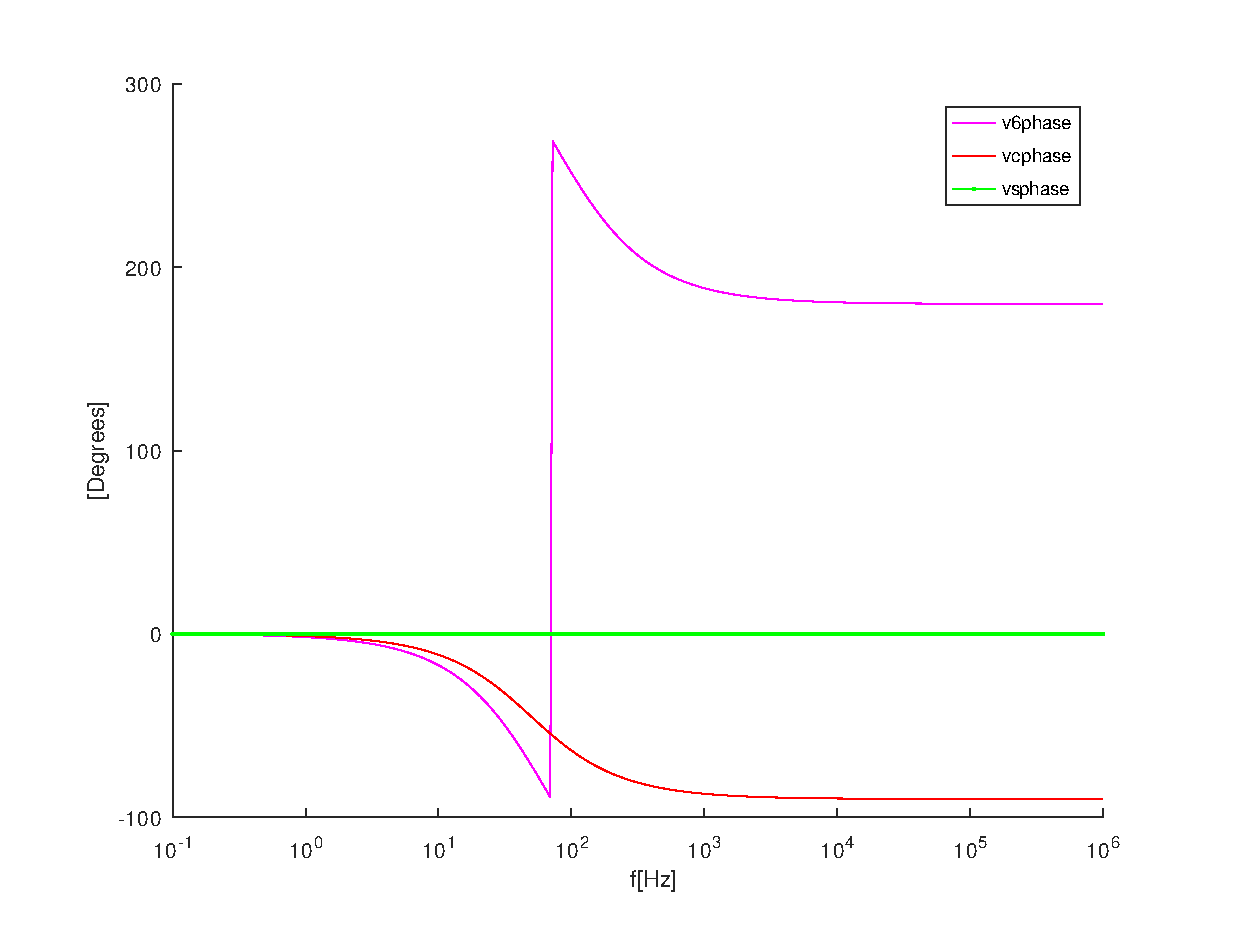
\includegraphics[width=0.6\textwidth]{phase.eps}
\caption{Phase $v_s(f)$,  $v_c(f)$  and $v_6(f)$ during frequency interval [0.1 , 1] MHz.}
\label{fig:phasetheo}
\end{figure}

The frequency $f$ is expressed in Hertz (Hz) along the x-axis and
the phase of $v_s(f)$,  $v_c(f)$  and $v_6(f)$ is expressed in degrees along the y-axis.\\
in this graph, the first thing that comes to the eye is the fact that the phase of $V_s$ will always be constant and that, once again, the $v_c$ graph line does not resemble the one that represents $v_6$. Last but not least, this graph illustrates very well the fact that, even though the node voltage in 6 will suddenly change, this discontinuoty will not have an effect on $V_c$, which must have a continous voltage, given that it is a capacitor.

